%This is paper.tex

%Write the contents of your paper here.

\newcommand{\degree}{$^\circ$}

\section{Introduction}
Tree volume measurement is one of the many parameters in documenting and 
profiling trees and is at the center of forest inventory. The use of this 
information is important to companies who need to make smart, profitable 
decisions but also need to be certain that the choices they make now are 
maintable in the future. However this information also benefits climate 
modellers, environmental groups and governments who want to be able to sustain 
ecosystems and plan restorations. To be able to accomplish this in forestry, 
it is a necessity to be able to collect large amounts of data easily and on a 
regular basis. Most methods used today to measure individual trees are often 
done manually with a variety of tools. The use of these analogue approaches 
is expensive, time consuming and in most cases the data collected doesn't meet 
today's standards \cite{digital imaged based tree measurement for forest inventory}. 
SilviaTerra, however, is a company willing to change that and have already 
developed several tools for scanning, analyzing and mapping areas of forestry 
to give accurate results. This is achieved through computer exactitude combined 
with statistical analysis. Recently a new project was started, with this 
research paper developing the mathematical back end, to allow users to easily 
get a correct volume measurement by only using their smart phone.

The measurements required for forest inventory can be achieved through a number 
of methods. One of them is using a so called biltmore stick. A biltmore stick 
is similar to a normal ruler but has been specially modified for measuring trees. 
When standing at a certain distance the user can discern the height of the tree 
by holding the biltmore stick up to their eye and reading the corresponding number. 
The biltmore stick can also easily be used to measure the DBH of the tree. 
Other ways of measuring tree volume include using a combination of lasers and 
inclinometers or by having a person manually climb up the tree and drop a tape 
measure down to measure the height. Despite these relatively simpe ways of 
measuring they often leave room for error. That’s why a more common way of 
getting a precise reading is to cut down trees in the area and then physically 
measure them. After the relevant data is collected one applies a stem-profile 
taper equation that is specific to the species of tree measured. These taper 
functions are based on numerous measurements and have been refined over the years. 
The main problem with taper functions is that to get an accurate result they 
need to be callibrated to the hundreds of local conditions. This again is cost 
prohibitive and only so much of a forest can be accounted for in the taper function. 
Even when one manages to create a new taper function, it is still far from 
perfect as all trees, even from the same species, differ in shape.

This project aims to solve the described problem by using a combination of 
photos taken of the tree, various sensor data from the phone and mathematical 
computation. This is supposed to then give a accurate result, cheaply and 
non-destructively. All within the reaches of a mobile phone.

\section{Background}

\begin{figure}[!htb]
	\minipage{0.45\textwidth}
		\centering
  		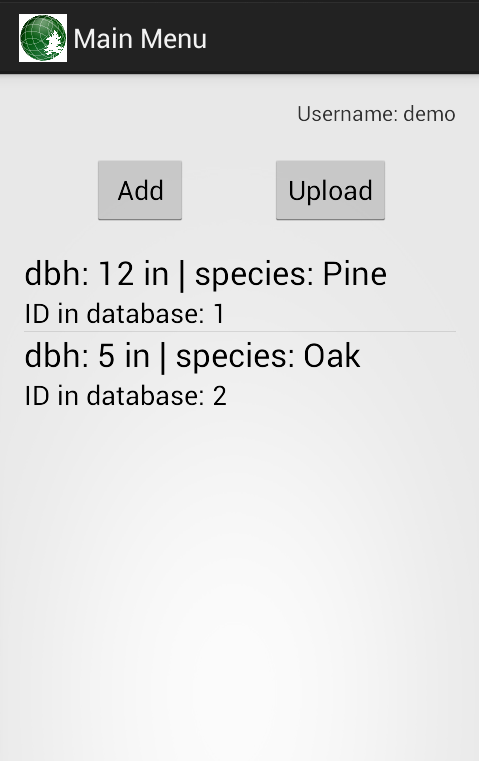
\includegraphics[width=0.65\textwidth]{main.png}
	  	\caption{Homescreen}
  		\label{main}
	\endminipage\hfill
	\minipage{0.45\textwidth}
		\centering
	  	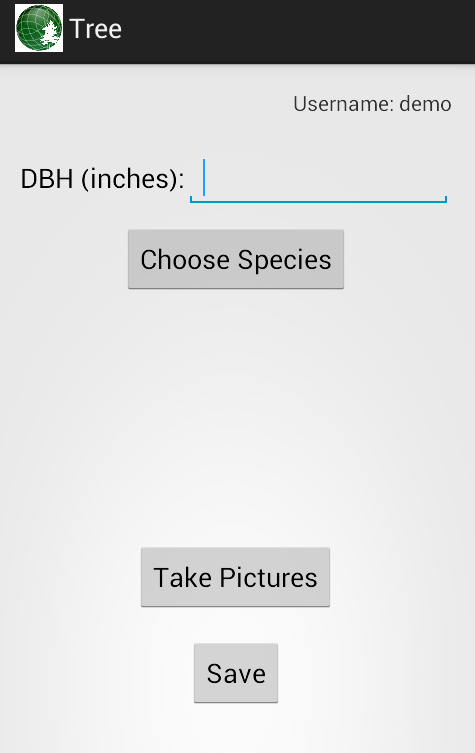
\includegraphics[width=0.65\textwidth]{input.png}
	  	\caption{User input}
  		\label{input}
	\endminipage\hfill
\end{figure}
The first thing a person does when accessing the mobile application is to log 
into the system with their user name and password. After that they are 
prompted with a simple menu where they can either choose to add new trees to 
their inventory or upload them to SilviaTerra's cloud service, figure \ref{main}. 
The data can then later be used with SilviaTerra's other products. If the user 
chooses to add a new tree then they will be asked to enter the tree's DBH and 
species, \ref{input}. 
\begin{figure}[!htb]
	\minipage{0.45\textwidth}
		\centering
  		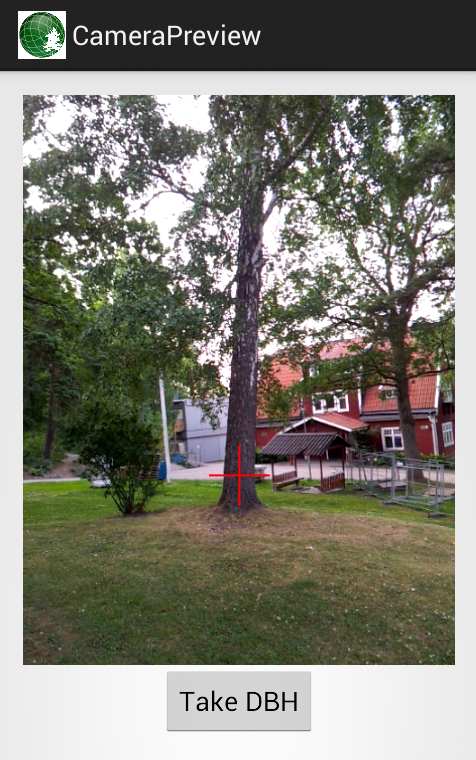
\includegraphics[width=0.75\textwidth]{dbh.png}
	  	\caption{DBH picture}
	  	\label{dbh}
	\endminipage\hfill
	\minipage{0.45\textwidth}
		\centering
	  	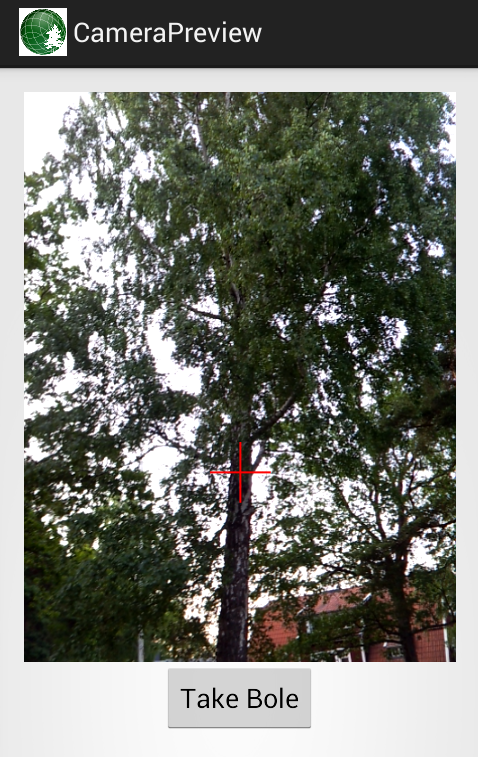
\includegraphics[width=0.75\textwidth]{bole.png}
	  	\caption{Bole picture}
	  	\label{bole}
	\endminipage\hfill
\end{figure}

After that they take two pictures. The interface is quite simple with a 
cross-hair to show where to point the camera. The first picture is of the 
actual DBH, figure \ref{dbh}, and the second picture is of the bole of the tree, 
figure \ref{bole}. Between these two pictures the camera will have to be tilted 
vertically to capture the bole. The angle between these two camera positions is 
recorded through the internal gyroscope. After this stage the user's role in 
the application is done and the pictures is sent to one of SilviaTerra's web 
servers. Here horizontal lines that run parallel with the bottom of the image 
are drawn across the entire picture. These are drawn at different pixel heights 
with equal pixel distance in between. The reason this is done is because 
computer vision is still an experimental technology and is not fully capable 
yet of being to detect the edges of trees with a background of forestry. 
Seeing as this is a commercial product, it would be quite disadvantageous if 
errors were commonplace. So instead the images with the newly drawn lines are 
then forwarded to Amazon's Mechanical Turk service. Just like the name suggests 
Amazon's Mechanical Turk is meant to be analogy to the 18th century concept of 
a automated chess board. The service is in its simplest form a crowd sourcing 
internet marketplace where individuals or businesses can request tasks to be 
completed. Usually the tasks are ones that are difficult for computers but 
easy for humans. SilviaTerra creates tasks where people manually click where 
the previously drawn lines, cross the edges of the tree. Ones of the points of 
intersection are identified, their corresponding pixel coordinates are the sent 
back to the web server. The pixel coordinates along with information from the 
phone is piped into a program where the volume is then calculated. It is this 
program that is the main topic of this research paper.

\section{Method}
Once all the required information has been retrieved it is piped into the 
program that will be calculating the volume. The dataset that is used comprises 
information about the phone and the results from Mechanical Turk. It is as follows:
\begin{itemize}
	\item DBH length
	\item Horizontal and vertical angle of view
	\item Horizontal and vertical image resolution
	\item Pitch of phone when images are captured
	\item Left and right pixel coordinates from Mechanical Turk
\end{itemize}

\subsection{Distance to tree}
The DBH is used as a reference to find all the other measurements. The first
unknown that must be discovered is the distance to the tree. This distance is 
parallel with the ground. The difference between the x-coordinates of the left 
and right pixel that correspond to the DBH is calculated, figure 
\ref{horizontal_triangle}, $X_1$ and $X_2$. Due to the fact that the width of
the DBH is now known in both pixels and in a physical measurement, the ratio
between the two can be determined by dividing the physical distance between 
$X_1$ and $X_2$ with the number of pixels betwee them.
\begin{figure}[htp]
\centering
{
	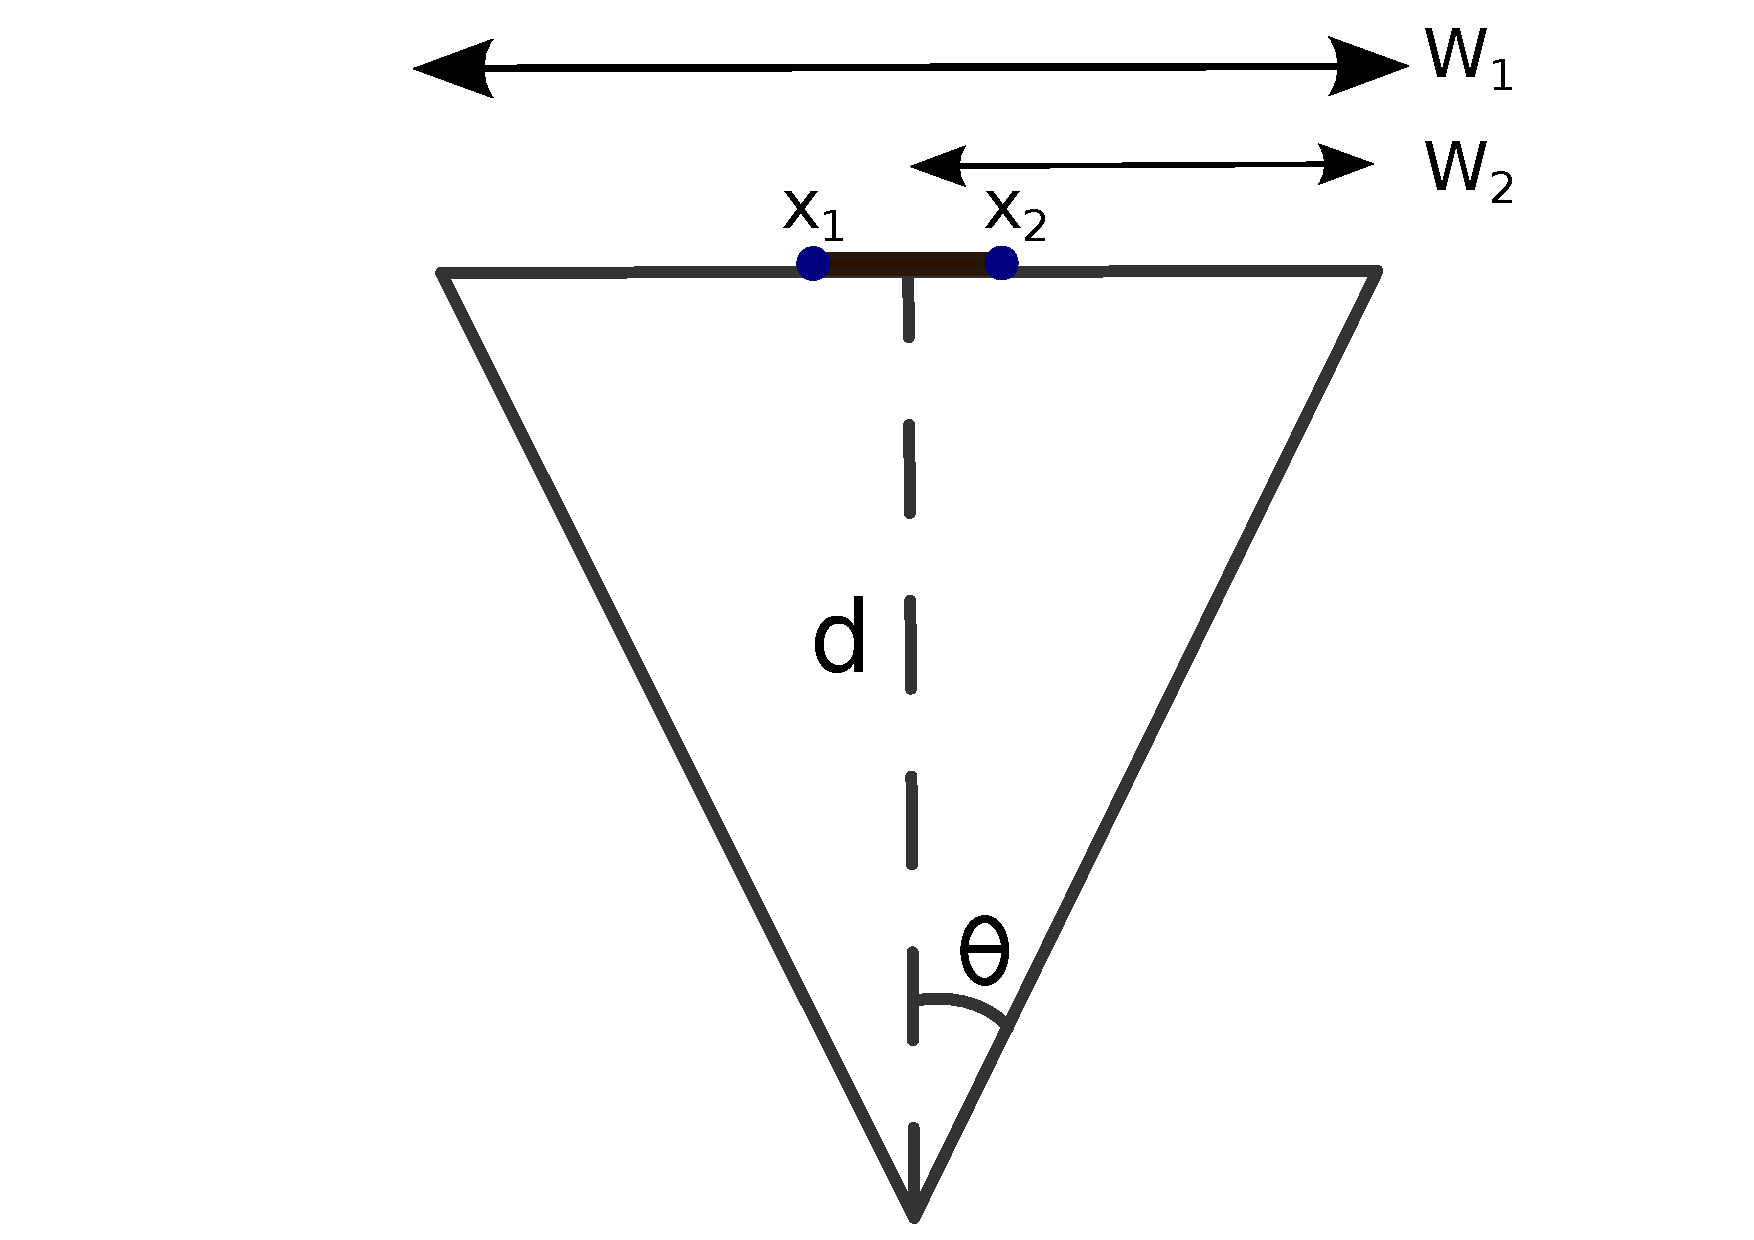
\includegraphics[scale=0.3]{horizontal_triangle.pdf}
	\caption{Birds eye view of horizontal plane}
	\label{horizontal_triangle}
}
\end{figure}
 As seen in figure \ref{horizontal_triangle} an isosceles triangle can be 
 constructed with the horizontal angle of view as the vertex angle. The triangles 
 two congruent legs extend out towards the base of the triangle, $W_1$, which 
 is inline with the tree. To get the length of the base, $W_1$, the previously 
 calculated scale between pixels and the real world is multiplied with the 
 number of pixels in the horizontal resolution of the image. The distance to 
 the tree can easily calculated by drawing an extra line that bisects the vertex
 angle, contriving the angle $\theta$ which is exactly half of the angle of view 
 and the actual distance to the tree $d$. This line also divides $W_1$ into $W_2$ 
 and futhermore producing a right angle triangle that can be solved. Finally to 
 actually calculate the distance, $d$, $W_2$ is divided by $\tan{\theta}$.


\subsection{Heights and widths} 
\begin{figure}[!htb]
	\minipage{0.45\textwidth}
		\centering
  		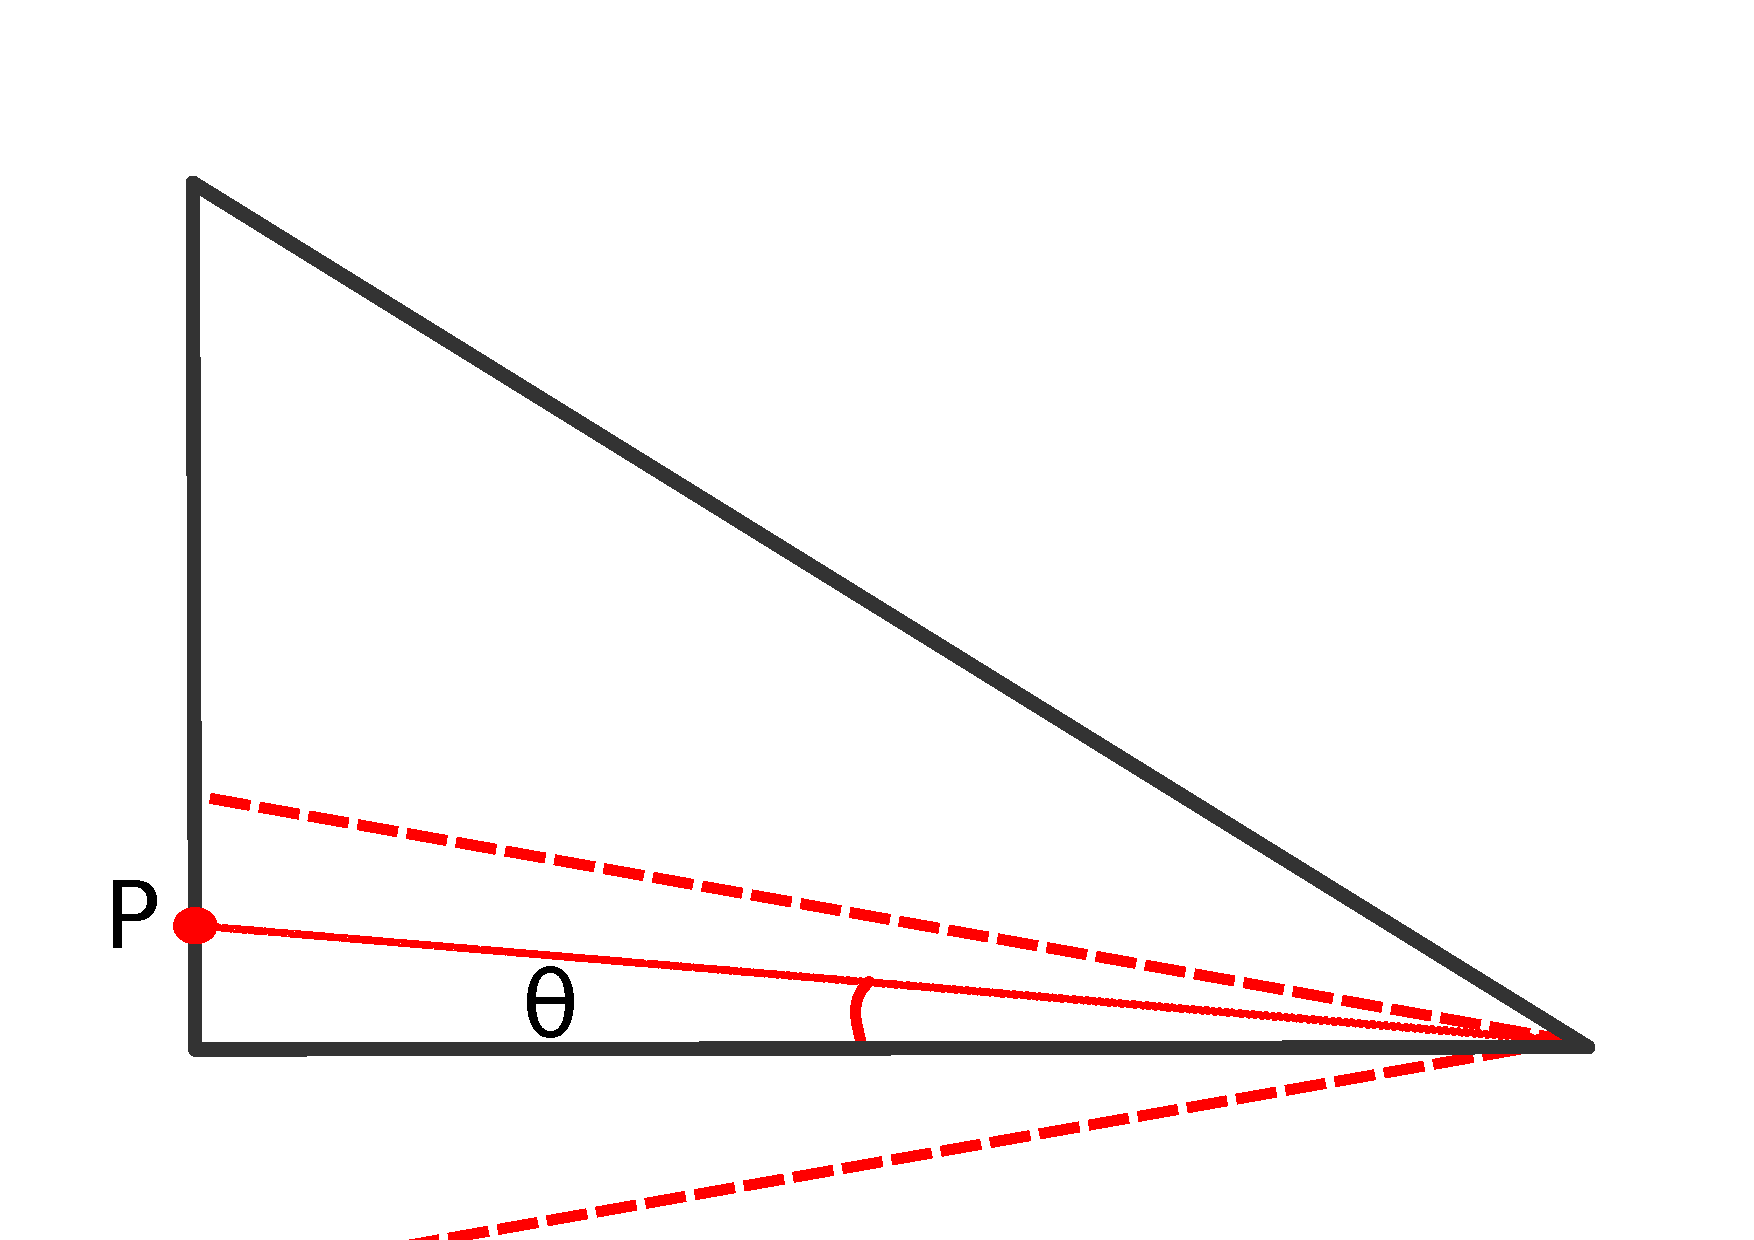
\includegraphics[width=0.9\textwidth]{triangle1.pdf}
	  	\caption{DBH picture}
	  	\label{triangle1}
	\endminipage\hfill
	\minipage{0.45\textwidth}
		\centering
	  	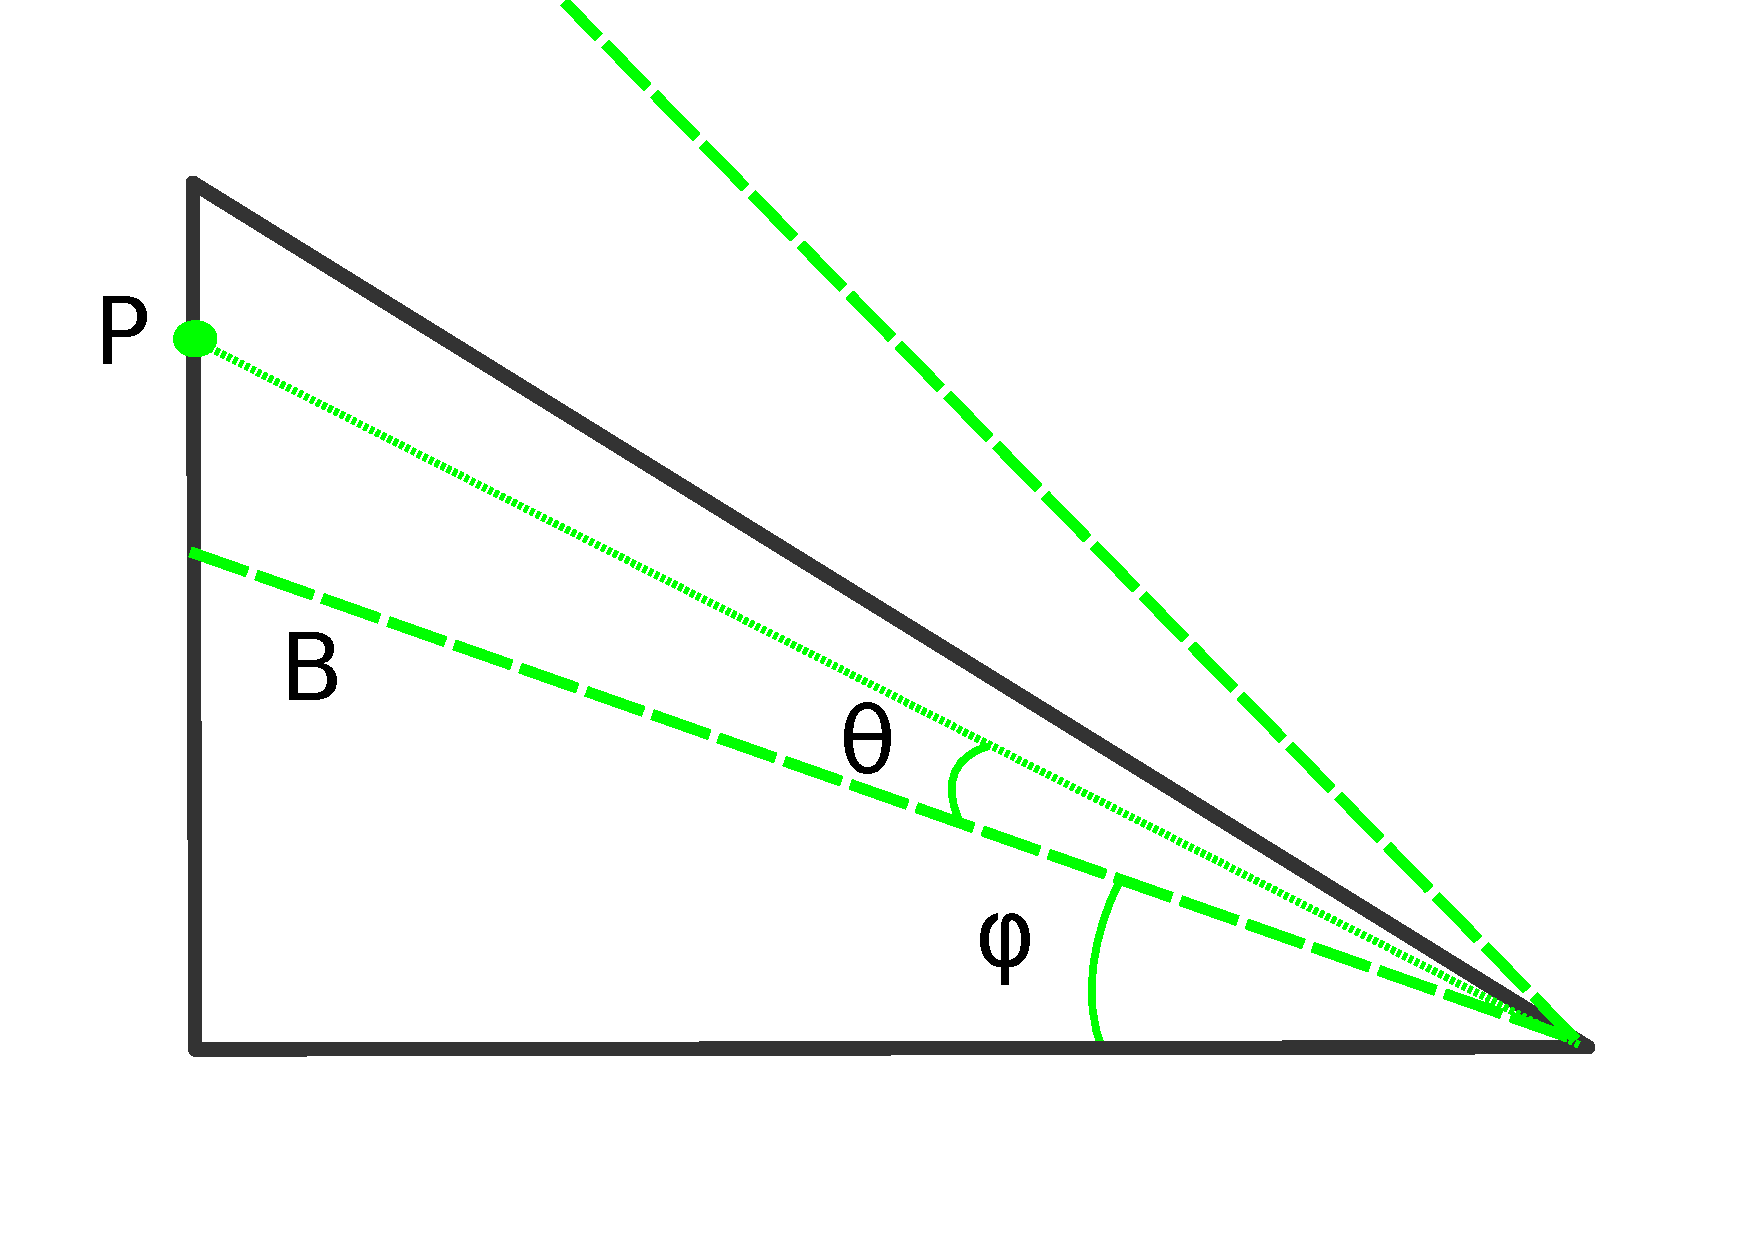
\includegraphics[width=0.9\textwidth]{triangle2.pdf}
	  	\caption{Bole picture}
	  	\label{triangle2}
	\endminipage\hfill
\end{figure}

The next stage is retrieving the real world height to each set pixel coordinates 
as well as the width between them, which will be the diameter of the tree. The 
first step taken is to get the height. The vertical image plate scale which is 
the ratio between degrees and pixels in the vertical axis is calculated by 
dividing the vertical resolution of the image with the vertical angle of view. 
This can be done because it is assumed that the silhouette of the tree is on a
plane in the real world which corresponds to the image plane. With this method 
it is possible to find out the angle to each pixel coordinate, $P$ in figure 
\ref{triangle1} and \ref{triangle2}, in the angle of view. This is angle is 
denoted by $\theta$ in both figure \ref{triangle1} and \ref{triangle2}. However 
if the pixel coordinate was identified in the second image, when the phone was 
tilted upwards, then angle between the distance to the tree and the lower boundary
of the vertical angle of view, $B$, will need to be added, which is represented
by $\varphi$ in figure \ref{triangle2}. The diagonal distance to $P$ is also 
calculated so that the width can later be determined.

The final part of obataining the parameters for the set of pixel coordinates at 
that height is to calculate the width between them. This is accomplished by 
employing the method for calculating the distance to the tree, in reverse. 
In this case what is known in figure \ref{horizontal_triangle} is the distance 
$d$ and the angle $\theta$ but not the width of the tree, $X_1$ to $X_2$. $W_2$ 
is calculated by multiplying $d$ with $\tan{\varphi}$. $W_2$ is then again 
multiplied by 2 and then divided by the number of pixels in the horizontal 
resolution of the image, once more returning the ratio between pixels and the 
corresponding real world measurement. To finish off this ratio is the multiplied
by the number of pixels between $X_1$ and $X_2$ dispensing the physical width
of the tree at that certain height.


\subsection{Volume}
Now the only thing left to produce the final result is to use these newly 
calculated widths and heights to obtain the total volume. The current implemented 
method of doing this is by integrating all the points using the trapezoidal rule.
All the widths are divided by 2 to get the radius. Then they are squared and
multiplied with $\pi$ to the obtain the basal area at each height. The basal 
area is plotted along with their corresponding heights. The trapezoidal rule 
then defines that the area between two points is: $\frac{a_1 + a_2}{2} \times h$.
The area between all the points is the summed together.


This whole process is looped through for every identified pixel coordinate set 
until the width and height is known for all of them. Once that is done, a new
loop is created for calculating the total volume.

\subsection{Simulation}
To test this method a \emph{virtual tree} was constructed. This tree was made 
out of blue tape and tapered off so that the program could be thoroughly tested. 
Along the tape points were marked out and the height to them plus the width
between corresponding points were measured. Just like in the real application, 
two pictures were taken. One of the DBH and one of the top of the tree. Each 
set of points was then identified on the pictures and measured in pixels. The 
parameters were then passed into the program and the results were cross-referenced
with the real life measurements.

\newpage

\section{Results}
\begin{table}[h!]
	\begin{center}
		\begin{tabular}{| l c c c c c c r |}		
		\hline
		Measured & 57\degree & 47\degree & 39\degree & 27\degree & 22\degree & 18\degree & 15\degree \\
		\hline
		0 		& 0 	& 0 	& 0 	& 0 	& 0 	& 0 	& 0 	\\
		103 	& 96 	& 100 	& 103 	& 106 	& 113 	& 116 	& 123 	\\
		115 	& 109 	& 113 	& 116 	& 118 	& 125 	& 128 	& 135 	\\
		125 	& 125 	& 129	& 132 	& 134 	& 140 	& 144 	& 150 	\\
		159 	& 142 	& 147 	& 150 	& 151 	& 158 	& 161 	& 167 	\\
		166 	& 158 	& 163 	& 166 	& 167 	& 174 	& 175 	& 183 	\\
		183 	& 173 	& 179 	& 181	& 182 	& 189 	& 192 	& 198 	\\
		\hline
		\end{tabular}
		\caption{Heights over DBH}
		\label{heights}
	\end{center}
\end{table}

\begin{table}[h!]
	\begin{center}
		\begin{tabular}{| l c c c c c c r |}
		\hline
		Measured & 57\degree & 47\degree & 39\degree & 27\degree & 22\degree & 18\degree & 15\degree \\
		\hline
		12       & 11.7      & 12.1      & 12.2      & 12.1      & 12.3      & 12.6      & 11.9      \\
		27       & 26.8      & 28.0      & 28.4      & 28.2      & 28.5      & 28.4      & 28.1      \\
		37       & 36.4      & 37.5      & 38.0      & 37.7      & 38.2      & 38.1      & 37.7      \\
		44       & 42.4      & 43.6      & 44.4      & 44.0      & 44.4      & 44.0      & 44.4      \\
		52       & 51.3      & 52.7      & 53.5      & 53.0      & 53.4      & 52.9      & 53.2      \\
		61       & 60.9      & 62.2      & 63.1      & 62.1      & 62.8      & 62.5      & 61.1      \\
		59       & 59.0      & 59.0      & 59.0      & 59.0      & 59.0      & 59.0      & 59.0      \\
		\hline
		\end{tabular}
		\caption{Widths over DBH}
		\label{widths}
    \end{center}
\end{table}

\begin{table}[h!]
	\begin{center}
    	\begin{tabular}{| l c c c c c c r |}
    	\hline
		Measured & 57\degree & 47\degree & 39\degree & 27\degree & 22\degree & 18\degree & 15\degree \\
		412222   & 386642    & 396386    & 418370    & 412084    & 433294    & 445401    & 445624    \\
		\hline
		\end{tabular}
		\caption{Total volume over DBH}
		\label{volumes}
    \end{center}
\end{table}
